\chapter{Cykly}

\indexItem{Prg}{cyklus \vb{while}}
Videli sme už príkazy na načítanie a vypísanie, uloženie výsledku do premennej
a vyhodnotenie podmienky. Ďalšie užitočné príkazy sú tzv. {\em cykly}, ktoré
nejaký príkaz opakujú viackrát. Predstavíme si jeden z nich: \prg~while~.
Príkaz \prg~while~ má, podobne ako \prg~if~, v zátvorkách napísanú
podmienku a za ňou príkaz. \prg ~while ~robí to, že stále dokola vyhodnocuje
podmienku a kým je splnená, vykonáva príkaz. Podobne ako pri \prg!if!
sa dá použiť zložený príkaz: v \prg!{}! uzavretých viac príkazov
sa správa ako jeden. Čo robí tento program?

\begin{lstlisting}
#include <iostream>
using namespace std;
int main() {
  int x;
  x = 1;
  while (x < 11) {
    cout << x << endl;
    x = x + 1;
  }
}
\end{lstlisting}

Najprv vyrobí premennú \prg~x~ a uloží do nej jednotku. Potom dokola robí toto:
\cmd{Pozri sa, či \prg~x < 11~. Ak áno, vypíš \prg~x~, ulož do \prg~x~ číslo
o 1 väčšie, ako tam bolo doteraz a celé to zopakuj.} Cyklus teda postupne vypíše riadky s 
číslami 1, 2, 3, 4, 5, 6, 7, 8, 9, 10 a potom skončí. Jedna vec, na ktorú si treba dávať pri 
cykle pozor, je, že sa ľahko môže stať, že nikdy neskončí a program sa {\em zacyklí}.
Keby sme napr. zabudli napísať riadok \prg~x = x + 1;~ \prg~x~ sa nikdy nezmení,
\prg~x < 11~ bude platiť stále a program bude donekonečna vypisovať riadok s číslom 1.

Urobme ešte jeden príklad. Dajme tomu, že najprv napíšeš jedno
prirodzené číslo $n$ a potom $n$ prirodzených čísel. Program má zistiť,
ktoré z nich je najväčšie. Napr. ak by si na vstupe napísal \prg!5 6 3 9 12 1!, 
program má vypísať \prg!12!.  Ako to naprogramovať? Najprv si vyrobíme
premennú \prg!int n;! kde si uložíme počet čísel \prg!cin >> n;! Potom
potrebujeme $n$-krát zopakovať toto: \cmd{Prečítaj číslo \prg!x!.  Ak je
väčšie, ako najväčšie číslo, ktoré sme doteraz videli, tak najväčšie videné číslo bude odteraz \prg!x!. Inak sa najväčšie videné číslo nezmení.} 
  Ako
môžme niečo zopakovať $n$-krát? Urobíme cyklus, v ktorom vždy odrátame z
\prg!n!  jednotku.  Keď nám v \prg!n! ostane nula, cyklus skončíme.

\begin{column}{0.6}
Naprogramovať zvyšok už nie je ťažké: budeme mať premennú \prg!int max;!
v ktorej si budeme pamätať doposiaľ najväčšie videné číslo. Vnútri cyklu načítame
jedno číslo zo vstupu a porovnáme ho s \prg!max!. Ostáva vyriešiť jediný problém:
čo dať na začiatku do premennej \prg~max~? A čo sa stane, ak do nej nedáme nič?
  \indexItem{Prg}{nedefinovaná hodnota}
V tom prípade hovoríme, že premenná má {\em nedefinovanú hodnotu} a to znamená, že 
v nej môže byť uložené čokoľvek. Nikdy nepíš program, ktorý používa premennú, do ktorej
predtým nič nezapísal. V našom prípade vieme, že budeš zadávať iba prirodzené čísla.
Keď teda na začiatku do \prg!max! uložíme nejaké záporné číslo, máme istotu,
že už prvé načítané číslo bude väčšie. 
\indexItem{Alg}{zarážka (sentinel)}
Toto je užitočná technika, ktorej sa hovorí 
{\em zarážka} ({\em sentinel}). 
Celý program teda bude vyzerať takto:
\end{column}
\hfill
\begin{column}{0.3}
\vbox{
\begin{lstlisting}
#include <iostream>
using namespace std;
int main() {
  int n, max, x;
  max = -1;
  cin >> n;
  while (n > 0) {
    cin >> x;
    if (x > max) max = x;
    n = n - 1;
  }
  cout << max << endl;
}
\end{lstlisting}
}
\end{column}

\begin{uloha}
  Používateľ napíše najprv jedno prirodzené číslo $n$
a potom $n$ prirodzených čísel. Napíš program, ktorý vypíše ich súčet.
\end{uloha}

\begin{column}{0.7}
\begin{uloha}
  Znova máme kamienky, tentokrát uložené do trojuholníka.
  Napíš program, ktorý prečíta zo vstupu jedno číslo: koľko kamienkov je v 
  spodnom riadku.
  Program má vypísať, koľko kamienkov je v celom trojuholníku. Vieš ho napísať aj bez 
  použitia cyklu?
\end{uloha}
\end{column}
\begin{column}{0.3}
  \centerline{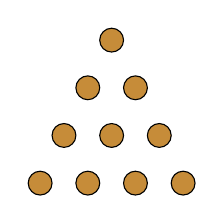
\begin{tikzpicture}
    \foreach \i in {0,...,3} \foreach \j in {0,...,\i}
    \filldraw[fill=brown!90!yellow] (\i*4ex-\j*2ex,\j*4ex) circle (1ex);
  \end{tikzpicture}}
\end{column}

\begin{uloha}
  Napíš program pre takúto úlohu.
  Používateľ postupne zadáva čísla. Keď napíše párne číslo, vypíš to isté číslo.
  Keď napíše nepárne, vypíš o jedno väčšie.
  Keď napíše \vb{-1}, program skončí.
\end{uloha}

\begin{uloha}
  Používateľ najprv zadá číslo $n$ a potom $n$ rôznych čísel. Napíš program, ktorý zistí,
  ako ďaleko sú od seba najväčšie a najmenšie číslo.
\end{uloha}

\begin{uloha}
  Používateľ najprv napíše prirodzené číslo $a$ a potom začne písať
  prirodzené čísla (nevieme, koľko). Nakoniec napíše -1.
  Napíš program, ktorý zistí, koľkokrát je medzi napísanými číslami
  číslo $a$. Napr. pre vstup \prg!3 9 3 8 7 3 6 6 7 3 3 7 8 -1!
  má byť odpoveď \prg!4!, lebo trojka sa v zadaných číslach 
  nachádza štyrikrát.
\end{uloha}

\begin{uloha}
  \label{uloha:collatz}
  Zoberme si takúto hru: mysli si číslo. Ak je párne, vydeľ ho dvoma. Ak je nepárne,
  vynásob ho tromi a pripočítaj 1. Toto opakuj, až kým sa nedostaneš k jednotke.
  Napríklad keď začneš s číslom $12$ budeš postupne dostávať čísla
  $6, 3, 10, 5, 16, 8, 4, 2, 1$.\footnote{V matematike je známa% 
  \indexItem{Mat}{Collatzova hypotéza}%
  Collatzova hypotéza, ktorá 
  hovorí, že nech začneš z hocijakého čísla, vždy sa nakoniec k jednotke dostaneš.
  Matematikov veľmi hnevá, že stále nevedia Collatzovu hypotézu dokázať.
  Na druhej strane, zatiaľ ani nenašli žiadne číslo, ktoré
  by sa po čase k jednotke nedostalo, a to už vyskúšali všetky čísla až po
  $295147905179352825856$. }

  Napíš program, ktorý prečíta zo vstupu jedno číslo a vypíše, ako dlho trvá, kým
  sa dostaneš k jednotke a aké najväčšie číslo pri tom stretneš. Pre $12$
  má program vypísať $9$ a $16$, lebo k jednote sa dostaneš po $9$ krokoch a 
  najväčšie číslo, ktoré stretneš je 16. Pre $27$ má vypísať $111$ a $9232$.

  (Zistiť, či je číslo párne, sa dá jednoducho pomocou operácie \vb{\%}, ktorá
  dáva zvyšok po delení. Ak teda chceš urobiť nejaký príkaz, iba ak \prg!n!
  je párne, stačí napísať \prg!if (n % 2 == 0) ...!)
\end{uloha}

\begin{uloha} Používateľ postupne zadáva čísla. Napíš program, ktorý
  po každom zadanom čísle vypíše súčet všetkých čísel od začiatku až doteraz.
  Keď používateľ zadá -1, program skončí.
\end{uloha}

\begin{uloha}
  \label{uloha:Fibonacci}
  \indexItem{Mat}{Fibonacciho čísla, zlatý rez}
  Fibonacciho čísla sú postupnosť čísel, ktorú vieme zostrojiť takto: prvé dve
  Fibonacciho čísla sú $0$, $1$. Ďalšie číslo vyrobím tak, že sčítam dve posledné.
  Celá postupnosť teda vyzerá $0,1,1,2,3,5,8,13,21,\ldots$.\footnote{%
   Fibonacciho čísla sú veľmi zaujímavé. Pomer dvoch za sebou idúcich Fibonacciho
   čísel sa blíži k
   tzv. {\em zlatému rezu}. V prírode sa často vyskytujú v rôznych útvaroch, 
   napr. pri špirálach:\newline\newline

    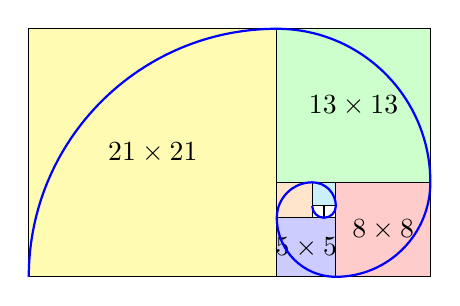
\begin{tikzpicture}[scale=0.15]
      \filldraw[fill=yellow!30!white] (0,0) rectangle node[anchor=center] {$21\times 21$} (21,21);
      \filldraw[fill=green!20!white] (21,21) rectangle node[anchor=center] {$13\times 13$} (34,8);
      \filldraw[fill=red!20!white] (26,8) rectangle node[anchor=center] {$8\times 8$} (34,0);
      \filldraw[fill=blue!20!white] (21,5) rectangle node[anchor=center] {$5\times 5$} (26,0);
      \filldraw[fill=orange!20!white] (21,8) rectangle  (24,5);
      \filldraw[fill=cyan!20!white] (24,8) rectangle  (26,6);
      \filldraw[fill=white] (24,6) rectangle  (25,5);

      \draw[thick,blue] (0,0) 
        arc[start angle=180, end angle=90, radius=21] 
        arc[start angle=90, end angle=0, radius=13] 
        arc[start angle=0, end angle=-90, radius=8] 
        arc[start angle=-90, end angle=-180, radius=5] 
        arc[start angle=180, end angle=90, radius=3] 
        arc[start angle=90, end angle=0, radius=2] 
        arc[start angle=0, end angle=-180, radius=1] 
;
    \end{tikzpicture}
    }
    Napíš program, ktorý pre zadané $n$ vyráta $n$-té Fibonacciho číslo.

\end{uloha}

\indexItem{Alg}{vnorené cykly}
Podobne ako podmienky, aj cykly môžu byť vnorené: príkaz, ktorý sa vykonáva v cykle,
môže opäť obsahovať cyklus. Pozrime na na takýto príklad: používateľ na vstupe napíše číslo
$n$. Program má vypísať šachovnicový vzor rozmerov $n\times n$, pričom sa v ňom
striedavo opakujú \prg!0!
a \prg!1!. Napríklad pre vstup \prg!5! by program vypísal

\begin{outputBox}
01010
10101
01010
10101
01010
\end{outputBox}

Ako naprogramovať niečo takéto? Začiatok je ľahký: budeme mať premennú \prg!int r!, v ktorej
vždy bude uložené, ktorý riadok robíme. Začneme s tým, že do nej uložíme nulu a v cykle
ju budeme postupne zväčšovať až po $n$. V rámci cyklu potrebujeme vypísať jeden riadok.
Riadok sa skladá z $n$ znakov, preto môžeme použiť inú premennú, \prg!int s!, v ktorej 
bude uložené, ktorý stĺpec v riadku práve robíme. Na začiatku riadku uložíme do
\prg!s! nulu a v cykle budeme $n$-krát pripočítavať jednotku 
a budeme striedavo vypisovať nulu
a jednotku. Vystriedame ich ľahko: ak \prg!x! je 0, tak \prg!1-x! je 1 a naopak.
Posledná otázka: ako zistíme prvý znak v riadku? Premenná \prg!r! udáva číslo riadku
(začína od 0), takže stačí na začiatku zobrať zvyšok po delení 2. Celý program vyzerá takto:\\

\vbox{
\begin{lstlisting}
#include <iostream>
using namespace std;
int main() {
  int r, s, x, n;
  cin >> n;
  r = 0;
  while (r < n) {    // tento cykus sa zopakuje raz pre každý riadok
    x = r % 2;       // x je začiatočný znak
    s = 0;           
    while (s < n) {  // tento cyklus vypisuje znaky v riadku
      cout << x;
      x = 1 - x;     // zmení vypisovaný znak
      s = s + 1;
    }                // koniec cyklu pre znaky v riadku
    cout << endl;    
    r = r + 1;
  }                  // koniec cyklu pre riadky
}
\end{lstlisting}
}

\begin{column}{0.5}
\begin{uloha}
  Napíš program, ktorý načíta jedno číslo $n$ a vypíše štvorec z núl 
  orámovaný jednotkami, ktorý má $n$ riadkov. Pre $n=5$ má vzor vyzerať takto:
\end{uloha}
\end{column}
\hfill
\begin{column}{0.2}
\vspace*{-2ex}
\begin{outputBox}
11111
10001
10001
10001
11111
\end{outputBox}
\end{column}

\begin{column}{0.5}
\begin{uloha}
  Napíš program, ktorý načíta jedno číslo $n$ a vypíše štvorec z núl 
  a jednotiek, ktorý má $n+1$ riadkov. Pre $n=5$ má vzor vyzerať takto:
\end{uloha}
\end{column}
\hfill
\begin{column}{0.2}
\vspace*{-2ex}
\begin{outputBox}
00000
00001
00011
00111
01111
11111
\end{outputBox}
\end{column}

\begin{column}{0.5}
\begin{uloha}
  Napíš program, ktorý načíta jedno číslo $n$ a vypíše trojuholníkový vzor z núl 
  a jednotiek, ktorý má $n$ riadkov. Pre $n=5$ má vzor vyzerať takto:
\end{uloha}
\end{column}
\hfill
\begin{column}{0.2}
\vspace*{-2ex}
\begin{outputBox}
000010000
000111000
001111100
011111110
111111111
\end{outputBox}
\end{column}
